\documentclass[a4paper]{report}
% Some basic packages
\usepackage[utf8]{inputenc}
\usepackage[T1]{fontenc}
\usepackage{textcomp}
\usepackage[english]{babel}
\usepackage{url}
\usepackage{graphicx}
\usepackage{float}
\usepackage{booktabs}
\usepackage{enumitem}

\pdfminorversion=7

% Don't indent paragraphs, leave some space between them
\usepackage{parskip}

% Hide page number when page is empty
\usepackage{emptypage}
\usepackage{subcaption}
\usepackage{multicol}
\usepackage{xcolor}

% Other font I sometimes use.
% \usepackage{cmbright}

% Math stuff
\usepackage{amsmath, amsfonts, mathtools, amsthm, amssymb}
% Fancy script capitals
\usepackage{mathrsfs}
\usepackage{cancel}
% Bold math
\usepackage{bm}
% Some shortcuts
\newcommand\N{\ensuremath{\mathbb{N}}}
\newcommand\R{\ensuremath{\mathbb{R}}}
\newcommand\Z{\ensuremath{\mathbb{Z}}}
\renewcommand\O{\ensuremath{\emptyset}}
\newcommand\Q{\ensuremath{\mathbb{Q}}}
\newcommand\C{\ensuremath{\mathbb{C}}}
\renewcommand\L{\ensuremath{\mathcal{L}}}

% Package for Petri Net drawing
\usepackage[version=0.96]{pgf}
\usepackage{tikz}
\usetikzlibrary{arrows,shapes,automata,petri}
\usepackage{tikzit}
\input{petri_nets_style.tikzstyles}

% Easily typeset systems of equations (French package)
\usepackage{systeme}

% Put x \to \infty below \lim
\let\svlim\lim\def\lim{\svlim\limits}

%Make implies and impliedby shorter
\let\implies\Rightarrow
\let\impliedby\Leftarrow
\let\iff\Leftrightarrow
\let\epsilon\varepsilon

% Add \contra symbol to denote contradiction
\usepackage{stmaryrd} % for \lightning
\newcommand\contra{\scalebox{1.5}{$\lightning$}}

% \let\phi\varphi

% Command for short corrections
% Usage: 1+1=\correct{3}{2}

\definecolor{correct}{HTML}{009900}
\newcommand\correct[2]{\ensuremath{\:}{\color{red}{#1}}\ensuremath{\to }{\color{correct}{#2}}\ensuremath{\:}}
\newcommand\green[1]{{\color{correct}{#1}}}

% horizontal rule
\newcommand\hr{
    \noindent\rule[0.5ex]{\linewidth}{0.5pt}
}

% hide parts
\newcommand\hide[1]{}

% si unitx
\usepackage{siunitx}
\sisetup{locale = FR}

% Environments
\makeatother
% For box around Definition, Theorem, \ldots
\usepackage{mdframed}
\mdfsetup{skipabove=1em,skipbelow=0em}
\theoremstyle{definition}
\newmdtheoremenv[nobreak=true]{definitie}{Definitie}
\newmdtheoremenv[nobreak=true]{eigenschap}{Eigenschap}
\newmdtheoremenv[nobreak=true]{gevolg}{Gevolg}
\newmdtheoremenv[nobreak=true]{lemma}{Lemma}
\newmdtheoremenv[nobreak=true]{propositie}{Propositie}
\newmdtheoremenv[nobreak=true]{stelling}{Stelling}
\newmdtheoremenv[nobreak=true]{wet}{Wet}
\newmdtheoremenv[nobreak=true]{postulaat}{Postulaat}
\newmdtheoremenv{conclusie}{Conclusie}
\newmdtheoremenv{toemaatje}{Toemaatje}
\newmdtheoremenv{vermoeden}{Vermoeden}
\newtheorem*{herhaling}{Herhaling}
\newtheorem*{intermezzo}{Intermezzo}
\newtheorem*{notatie}{Notatie}
\newtheorem*{observatie}{Observatie}
\newtheorem*{exe}{Exercise}
\newtheorem*{opmerking}{Opmerking}
\newtheorem*{praktisch}{Praktisch}
\newtheorem*{probleem}{Probleem}
\newtheorem*{terminologie}{Terminologie}
\newtheorem*{toepassing}{Toepassing}
\newtheorem*{uovt}{UOVT}
\newtheorem*{vb}{Voorbeeld}
\newtheorem*{vraag}{Vraag}

\newmdtheoremenv[nobreak=true]{definition}{Definition}
\newtheorem*{eg}{Example}
\newtheorem*{notation}{Notation}
\newtheorem*{previouslyseen}{As previously seen}
\newtheorem*{remark}{Remark}
\newtheorem*{note}{Note}
\newtheorem*{problem}{Problem}
\newtheorem*{observe}{Observe}
\newtheorem*{property}{Property}
\newtheorem*{intuition}{Intuition}
\newmdtheoremenv[nobreak=true]{prop}{Proposition}
\newmdtheoremenv[nobreak=true]{theorem}{Theorem}
\newmdtheoremenv[nobreak=true]{corollary}{Corollary}

% End example and intermezzo environments with a small diamond (just like proof
% environments end with a small square)
\usepackage{etoolbox}
\AtEndEnvironment{vb}{\null\hfill$\diamond$}%
\AtEndEnvironment{intermezzo}{\null\hfill$\diamond$}%
% \AtEndEnvironment{opmerking}{\null\hfill$\diamond$}%

% Fix some spacing
% http://tex.stackexchange.com/questions/22119/how-can-i-change-the-spacing-before-theorems-with-amsthm
\makeatletter
\def\thm@space@setup{%
  \thm@preskip=\parskip \thm@postskip=0pt
}


% Exercise 
% Usage:
% \exercise{5}
% \subexercise{1}
% \subexercise{2}
% \subexercise{3}
% gives
% Exercise 5
%   Exercise 5.1
%   Exercise 5.2
%   Exercise 5.3
\newcommand{\exercise}[1]{%
    \def\@exercise{#1}%
    \subsection*{Exercise #1}
}

\newcommand{\subexercise}[1]{%
    \subsubsection*{Exercise \@exercise.#1}
}


% \lecture starts a new lecture (les in dutch)
%
% Usage:
% \lecture{1}{di 12 feb 2019 16:00}{Inleiding}
%
% This adds a section heading with the number / title of the lecture and a
% margin paragraph with the date.

% I use \dateparts here to hide the year (2019). This way, I can easily parse
% the date of each lecture unambiguously while still having a human-friendly
% short format printed to the pdf.

\usepackage{xifthen}
\def\testdateparts#1{\dateparts#1\relax}
\def\dateparts#1 #2 #3 #4 #5\relax{
    \marginpar{\small\textsf{\mbox{#1 #2 #3 #5}}}
}

\def\@lecture{}%
\newcommand{\lecture}[3]{
    \ifthenelse{\isempty{#3}}{%
        \def\@lecture{Lecture #1}%
    }{%
        \def\@lecture{Lecture #1: #3}%
    }%
    \subsection*{\@lecture}
    \marginpar{\small\textsf{\mbox{#2}}}
}



% These are the fancy headers
\usepackage{fancyhdr}
\pagestyle{fancy}

% LE: left even
% RO: right odd
% CE, CO: center even, center odd
% My name for when I print my lecture notes to use for an open book exam.
% \fancyhead[LE,RO]{Gilles Castel}

\fancyhead[RO,LE]{\@lecture} % Right odd,  Left even
\fancyhead[RE,LO]{}          % Right even, Left odd

\fancyfoot[RO,LE]{\thepage}  % Right odd,  Left even
\fancyfoot[RE,LO]{}          % Right even, Left odd
\fancyfoot[C]{\leftmark}     % Center

\makeatother




% Todonotes and inline notes in fancy boxes
\usepackage{todonotes}
\usepackage{tcolorbox}

% Make boxes breakable
\tcbuselibrary{breakable}

% Verbetering is correction in Dutch
% Usage: 
% \begin{verbetering}
%     Lorem ipsum dolor sit amet, consetetur sadipscing elitr, sed diam nonumy eirmod
%     tempor invidunt ut labore et dolore magna aliquyam erat, sed diam voluptua. At
%     vero eos et accusam et justo duo dolores et ea rebum. Stet clita kasd gubergren,
%     no sea takimata sanctus est Lorem ipsum dolor sit amet.
% \end{verbetering}
\newenvironment{verbetering}{\begin{tcolorbox}[
    arc=0mm,
    colback=white,
    colframe=green!60!black,
    title=Opmerking,
    fonttitle=\sffamily,
    breakable
]}{\end{tcolorbox}}

% Noot is note in Dutch. Same as 'verbetering' but color of box is different
\newenvironment{noot}[1]{\begin{tcolorbox}[
    arc=0mm,
    colback=white,
    colframe=white!60!black,
    title=#1,
    fonttitle=\sffamily,
    breakable
]}{\end{tcolorbox}}




% Figure support as explained in my blog post.
\usepackage{import}
\usepackage{xifthen}
\usepackage{pdfpages}
\usepackage{transparent}
\newcommand{\incfig}[1]{%
    \def\svgwidth{\columnwidth}
    \import{./figures/}{#1.pdf_tex}
}

% Fix some stuff
% %http://tex.stackexchange.com/questions/76273/multiple-pdfs-with-page-group-included-in-a-single-page-warning
\pdfsuppresswarningpagegroup=1


% My name
\author{Bruno M. Pacheco}

 
\begin{document}
 
\title{Lista 2}
\author{Bruno M. Pacheco\\
DAS 5142 - Sistemas Dinâmicos}
 
\maketitle
 
\exercise{1}

\subexercise{a}

\[
\bm{x} = \begin{bmatrix} \theta \\ \dot{\theta} \end{bmatrix} \implies \begin{cases}
    \dot{x_1} = x_2 \\
    \dot{x_2} = \frac{1}{J}u
\end{cases}
.\] 

Os estados variam como se sob a ação de dois sistemas diferentes limitados pela superfície definida por $e = 0$ de forma que as duas regiões levam o estado para a superfície de comutação, convergindo para o equilíbrio.

\subexercise{b}

\begin{figure}[H]
    \centering
    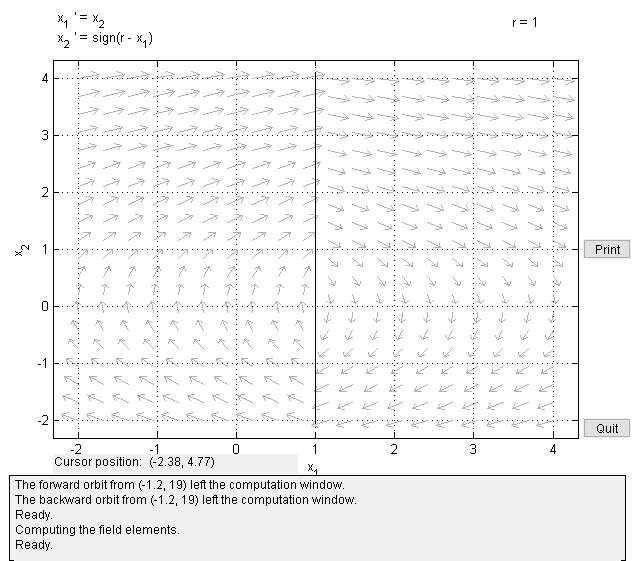
\includegraphics[width=0.8\textwidth]{lista2_1b.png}
    \caption{Diagrama de espaço de estados do sistema com superfície de deslizamento representada pela linha.}
    \label{fig:lista2_1b-png}
\end{figure}

Como o sistema é tal que \[
L_f^{+} = L_f^{-} = -x_2
\] o sistema não possui região de deslizamento e fica comutando enquanto converge para o equilíbrio em $(\theta_r,0)$. Isso é visível pela figura através da representação do seu campo.

\subexercise{c}

Utilizando a lei de controle $e = \theta_r - \theta - \dot{\theta}$, temos que \[
\begin{cases}
    L_f^{+} = -x_2-\frac{1}{J} \\
    L_f^{-} = -x_2 + \frac{1}{J}
\end{cases}
,\] portanto a região de deslizamento se dá para $x_2 \in \left[ -\frac{1}{J},\frac{1}{J} \right]$. Ainda mais, \[
x_2 in \left( -\frac{1}{J}, \frac{1}{J} \right) \implies L_f^{+}<0<L_f^{-}
,\] portanto o equilíbrio em $(\theta_r, 0)$ é estável.

\begin{figure}[H]
    \centering
    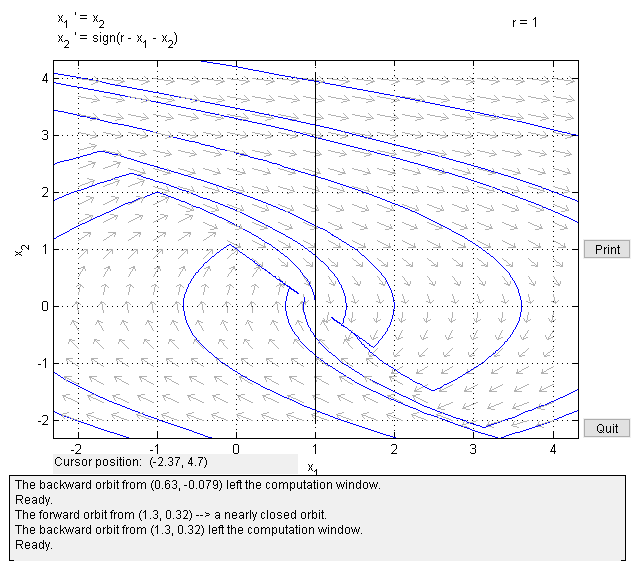
\includegraphics[width=0.8\textwidth]{lista2_1c.png}
    \caption{Diagrama de estados do sistema com a nova lei de controle que inclui amortecimento.}
    \label{fig:lista2_1c-png}
\end{figure}

\subexercise{d}

Podemos aproximar o efeito da comutação por uma lei de controle \[
u = \frac{e}{\pm\sqrt{e^2 + \epsilon^2} }
\] com $\epsilon$ suficientemente pequeno, de forma que a resposta seja mais suave, ou seja, sem incluir frequências tão altas e, portanto, mitigando o efeito do \emph{chattering}.

\exercise{2}

Representamos o sistema através dos estados \[
\begin{cases}
    x_1 = \theta \\
    x_2 = \dot{p} \\
    x_3 = \dot{\theta}
\end{cases}
.\] Assim, podemos escrever
\begin{align*}
    \begin{bmatrix} M_t & -ml\cos x_3 \\ -ml\cos x_3 & J_t \end{bmatrix} \begin{bmatrix} \dot{x_2} \\ \dot{x_3} \end{bmatrix} &= \begin{bmatrix} 
    -cx_2 -ml\sin(x_1)x_3^2 + F \\
    -\gamma x_3 + mgl\sin x_1
\end{bmatrix} \\
    \implies \begin{bmatrix} \dot{x_2} \\ \dot{x_3} \end{bmatrix} &= \begin{bmatrix} M_t & -ml\cos x_3 \\ -ml\cos x_3 & J_t \end{bmatrix}^{-1} \begin{bmatrix} 
    -cx_2 -ml\sin(x_1)x_3^2 + F \\
    -\gamma x_3 + mgl\sin x_1
\end{bmatrix} \\
								  &= \frac{1}{d}\begin{bmatrix} J_t & ml\cos x_3 \\ ml\cos x_3 & M_t \end{bmatrix} \begin{bmatrix} 
    -cx_2 -ml\sin(x_1)x_3^2 + F \\
    -\gamma x_3 + mgl\sin x_1
\end{bmatrix} \tag{*} \\
,\end{align*} onde $d = J_tM_t - m^2l^2\cos^2x_3$.

\subexercise{b}

No equilíbrio, temos
\begin{align*}
    & \dot{x_1} = 0 \implies x_3 = 0 \\
    \implies &(*): \begin{bmatrix} 0\\0 \end{bmatrix} = \frac{1}{d}\begin{bmatrix} J_t & ml \\ ml & M_t \end{bmatrix} \begin{bmatrix} 
    -cx_2 -ml\sin(x_1) + F \\
    mgl\sin x_1
\end{bmatrix}  \\
    \implies & \begin{bmatrix} 0 \\ 0 \end{bmatrix} = \begin{bmatrix} 
    -cx_2 -ml\sin(x_1) + F \\
    mgl\sin x_1
\end{bmatrix} \\
    \implies & \sin x_1 = 0 \implies x_1 \in \left\{ 0, \pi \right\} \\
    \implies & 0 = -cx_2 -ml\sin x_1 \implies x_2 = 0
,\end{align*} ou seja, existe equilíbrio em $(0,0,0)$ e $(\pi,0,0)$. Caso haja ação de controle, existe equilíbrio em $x_2 = \frac{F}{c}$.

Podemos expandir nosso sistema como \[
\begin{bmatrix} \dot{x_1} \\ \dot{x_2} \\ \dot{x_3} \end{bmatrix} = \frac{1}{d} \begin{bmatrix} 
x_2 d \\
J_t\left( -cx_2 -ml\sin(x_1)x_3^2 + F \right) + ml\cos x_3 \left( -\gamma x_3 + mgl\sin x_1 \right) \\
ml\cos x_3\left( -cx_2 -ml\sin(x_1)x_3^2 + F \right) + M_t \left( -\gamma x_3 + mgl\sin x_1 \right) \\
\end{bmatrix}
,\] o que nos permite calcular
\begin{align*}
J = \frac{1}{d}\begin{bmatrix} 
    0 & d & 0 \\
    ml\cos x_1 \left( mlg\cos x_3 -J_t x_3^2 \right) & -J_t c & -2 J_t ml \sin(x_1)x_3 + ml\gamma(\sin(x_3)x_3 -\cos(x_3)) \\
    ml \cos(x_1) \left( ml\cos(x_3)x_3^2 + M_t g \right) & -cml\cos x_3 & mlcx_2\sin x_3 -m^2l^2\sin x_1 \left( -\sin (x_3)x_3^2 + 2\cos (x_3)x_3 \right) -\gamma M_t 
\end{bmatrix} \\
\implies J(0,0,0) = \begin{bmatrix} 
    0 & d & 0 \\
    m^2l^2g & -J_t c & -ml\gamma \\
    M_t mlg & -cml & 
\end{bmatrix}  \\
.\end{align*}

\exercise{3}

Para a função candidata enunciada,
\begin{align*}
    \dot{V} &= -\sin x_1 \dot{x_1} +2a \cos x_1 \sin x_1 \dot{x_1} + x_2 \dot{x_2} \\
	    &= \sin x_1\left( 2a\cos x_1 - 1 \right) \dot{x_1} + x_2 \dot{x_2} \\
	    &= \sin x_1\left( 2a\cos x_1 - 1 \right) x_2 + x_2 \left( \sin x_1 + u \cos x_1 \right)  
.\end{align*}
Substituindo a lei de controle proposta,
\begin{align*}
    \dot{V} &= x_2 \left( \sin x_1\left( 2a\cos x_1 - 1 \right) + \sin x_1 -2a \sin x_1 \cos x_1 -x_2 \cos^2 x_1\right) \\
	    &= -x_2^2\cos^2x_1
.\end{align*}
Assim, podemos concluir que $\dot{V}$ é estritamente negativa definida em $x_1 \in \left( -\frac{\pi}{2}, \frac{\pi}{2} \right)$, sendo somente semi-negativa definida no restante do espaço. Portanto, o sistema é localmente assintoticamente estável, mas globalmente estável.

\exercise{4}

\subexercise{a}

Utilizando como estados $x = \varphi$ e $y=\dot{\varphi}$, temos pela equação (1) \[
I\dot{y} + by = u \implies \begin{cases}
    \dot{x} = y \\
    \dot{y} = u - by
\end{cases}
.\] O sistema funciona de forma análoga ao já explicado na questão 1a).

\subexercise{b}

O controle através da superfície $h=0$ se dá de forma que \[
    \nabla h = \begin{bmatrix} -k_p & -k_d \end{bmatrix} \implies \begin{cases}
    L_f^{+} = -k_p y +k_d b y -k_d < 0 \forall y < \frac{k_d}{bk_d-k_p} \\
    L_f^{-} = -k_p y +k_d b y +k_d > 0 \forall y > \frac{-k_d}{bk_d-k_p} \\
\end{cases}
.\] Assim, afirmamos que a região de deslizamento se dá para $y \in \left[ -\frac{k_d}{b k_d-k_p}, \frac{k_d}{b k_d-k_p} \right] $ e é estável fora das extremidades desse intervalo. Veja que, se $k_d = k_p = 1$, a região de deslizamento se torna $\left[ -\frac{1}{b-1}, \frac{1}{b-1} \right] $, ainda estável para $b>1$.

Agora, para os pseudo-equilíbrios, temos
\begin{align*}
    0 &= L_f^{+}f^{-} - L_f^{-}f^{-} \\
    &= \begin{bmatrix} 
	(-k_p +b k_d ) y^2 -k_d y  \\
	(k_p -b k_d ) by^2 -k_p y - k_d
    \end{bmatrix} - \begin{bmatrix} 
	(-k_p +b k_d ) y^2 -k_d y  \\
	(-k_p +b k_d ) by^2 +(-k_p +2bk_d) y - k_d
    \end{bmatrix} \\
    &= \begin{bmatrix} 
	0 \\
	2b\left( k_p -bk_d \right) y^2 -2bk_d y
    \end{bmatrix} \tag{*} \\
    &= \begin{bmatrix} 
	0 \\
	2b y\left( \left( 1-b \right) y -1 \right) 
    \end{bmatrix} \\
    &\implies y \in \left\{  0, \frac{1}{1-b}\right\} 
.\end{align*}
Entretanto, o ponto de equilíbrio em $y= \frac{1}{1-b}$ é a extremidade da região de deslizamento, fora da zona de estabilidade. Na superfície de deslizamento, o equilíbrio em $y=0$ significa o equilíbrio em $(\varphi_r,0)$, que é estável pelos limites encontrados.

\begin{figure}[H]
    \centering
    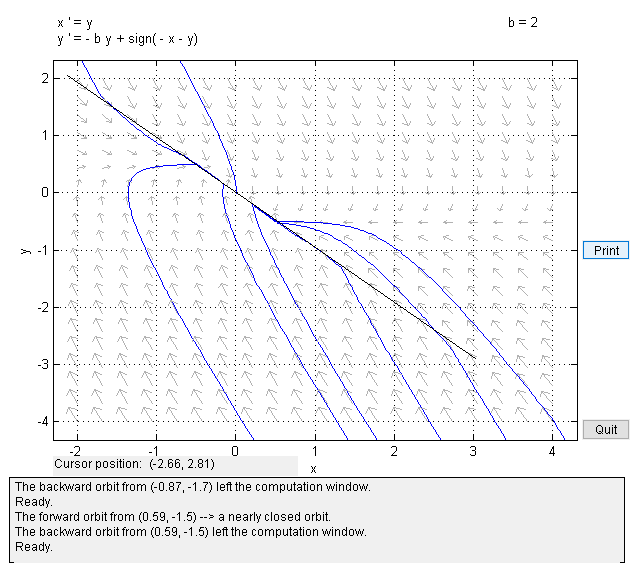
\includegraphics[width=0.6\textwidth]{lista2_4b.png}
    \caption{Diagrama de estados do sistema com $k_p = k_d = 1$.}
    \label{fig:lista2_4b-png}
\end{figure}

\subexercise{c}

Veja que $k_d=0$ resulta em uma região de deslizamento que inclui somente o ponto em $y=0$ e que não é estável. Vemos o resultado no diagrama de estados abaixo: o sistema não possui região de deslizamento. A solução, então, para a equação (*) se torna somente o equilíbrio trivial.

\begin{figure}[H]
    \centering
    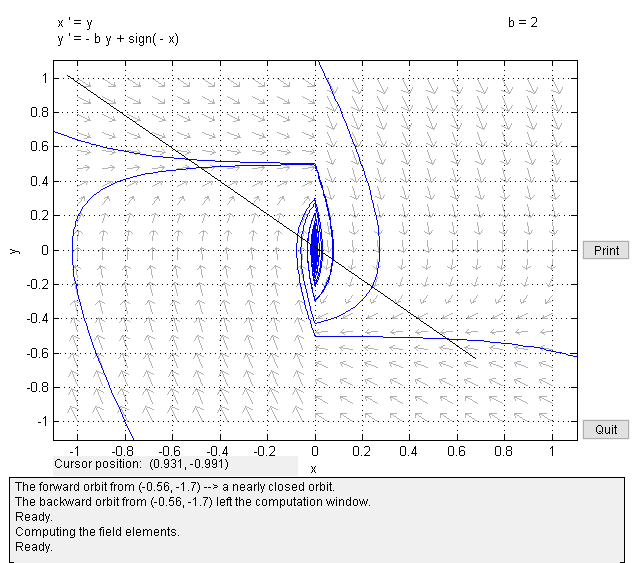
\includegraphics[width=0.6\textwidth]{lista2_4c.png}
    \caption{Diagrama de estados do sistema com $k_d=0$.}
    \label{fig:lista2_4c-png}
\end{figure}

\subexercise{d}

Agora vemos que a região que antes era de deslizamento se torna repulsiva, uma vez que as condições de estabilidade  \[
    \begin{cases}
	L_f^{+} = -y -b y +1 < 0 \forall y > \frac{1}{b+1} \\
	L_f^{-} = - y - b y -1 > 0 \forall y > \frac{-1}{b+1} \\
    \end{cases}   
\] não se cumprem dentro da zone de deslizamento demarcada por $L_f^{-}L_f^{+} \le 0$.

\begin{figure}[H]
    \centering
    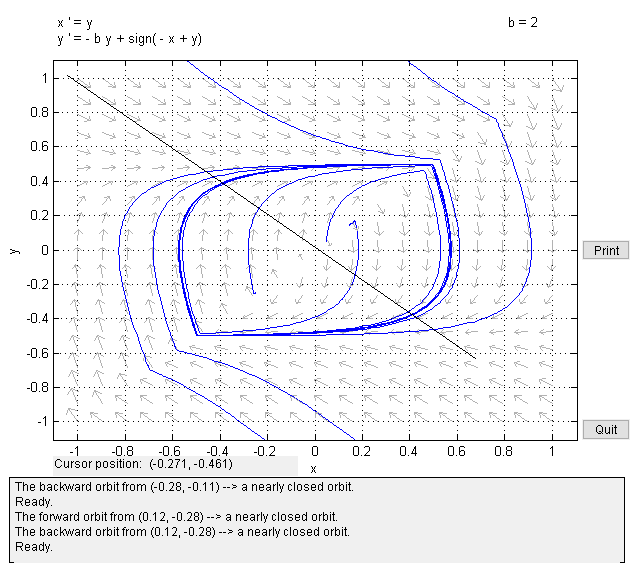
\includegraphics[width=0.6\textwidth]{lista2_4d.png}
    \caption{Diagrama de estados do sistema com $k_d=-1$}
    \label{fig:lista2_4d-png}
\end{figure}

\subexercise{e}

Vide exercício 1d).

\exercise{5}

Primeiro podemos analisar o sistema na perspectiva de espaço de estados, ou seja, utilizando \[
\begin{bmatrix} x_1 \\ x_2 \end{bmatrix} = \begin{bmatrix} \theta \\ \dot{\theta} \end{bmatrix} 
,\] podemo chegar no sistema \[
\begin{cases}
    \dot{x_1} = x_2 \\
    \dot{x_2} = \sin x_1 + u \cos x_1
\end{cases}
.\]  

Agora, verificamos a estabilidade do sistema utilizando a função de energia como função de Lyapunov, ou seja, verificamos que $\dot{V}$ é negativa definida no ponto $(0,0)$, posição vertical. Vejamos primeiro que \[
    V(\bm{x}) = \cos x_1 - 1 + \frac{1}{2}x_2^2
.\] Assim, utilizando a lei de controle proposta,
\begin{align*}
    \dot{V} &= \nabla V f(\bm{x}) = \begin{bmatrix} -\sin x_1 & x_2 \end{bmatrix} \begin{bmatrix} x_2 \\ \sin x_1 + u \cos x_1 \end{bmatrix} \\
    &= -x_2\sin x_1 + x_2 \sin x_1 + ux_2\cos x_1 \\
    &= k\left( V_0 -V \right) x_2^2 \cos^2 x_1 \\
    V_0 = V(0,0) = 0 &\implies \dot{V} = -kVx_2^2\cos^2x_1
,\end{align*}
o que nos mostra que, sendo $V$ positiva definida em $(0,0)$, o sistema é estável. Entretanto, $V$ não é positiva definida em $(0,0)$, então o sistema não é estável na posição vertical.

\exercise{6}

\subexercise{a}

Primeiro transformamos o sistema no espaço de estados como \[
\begin{cases}
    \dot{x_1} = x_2 \\
    m \dot{x_2} = u - b sign(x_2) -kx_1^3
\end{cases}
.\] Então, determinamos nossa função linearizante definindo uma nova entrada $v(t)$ para a planta, ou seja,
\begin{align*}
    &m v(t) = u(t) - b sign(x_2) - kx_1^3 \\
    &\implies u(t) = mv(t) + bsign\left( x_2 \right) +k x_1^3
.\end{align*}
Dessa forma, o sistema agora pode ser descrito como \[
\ddot{x}(t) = v(t)
.\] 

Veja que esse sistema é um duplo integrador, então fechando a malha com um controlador PD temos \[
    \frac{X}{R}(s) = \frac{K_p + sK_d}{s^2 + K_d s + K_p}
,\] ou seja, definindo $K_p = 1$ e  $K_d = 2\cdot 0,707$ teremos precisamente a resposta desejada.

\subexercise{b}

\begin{figure}[H]
    \centering
    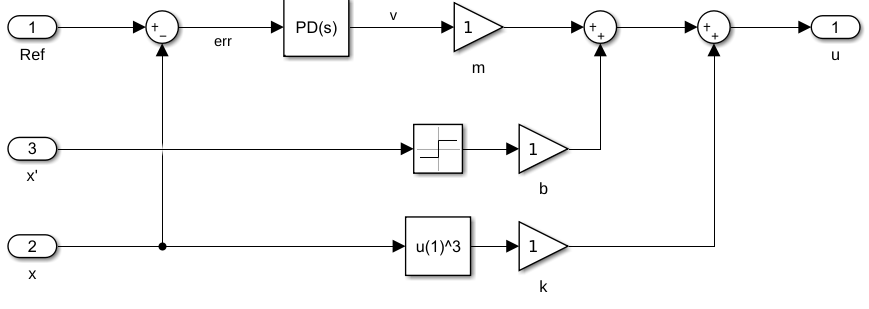
\includegraphics[width=0.8\textwidth]{lista2_6b.png}
    \caption{Diagrama de blocos do sistema de controle.}
    \label{fig:lista2_6b-png}
\end{figure}

\subexercise{c}

No espaço de estados, escrevemos \[
    V(x_1, x_2) = \frac{1}{4}k x_1^{4} + \frac{1}{2}mx_2^2
,\] que é claramente positiva definida no ponto de equilíbrio desejado.

Agora, queremos que $\dot{V}$ seja negativa definida, ou seja, 
\begin{align*}
    \dot{V} &= \nabla V f(x_1,x_2) = \begin{bmatrix} kx_1^3 & mx_2 \end{bmatrix} \begin{bmatrix} x_2 \\  \left(  u - b sign(x_2) - kx_1^3   \right) m^{-1} \end{bmatrix} \\
    &= ux_2 -x_2bsign(x_2) = u x_2 - b x_2 = \left( u - b \right) x_2
.\end{align*}
Se definirmos $u = -2b sign(x_2)$ garantimos que $\dot{V}$ seja negativa definida e, portanto, o sistema é estável em $(0,0)$.

\exercise{7}

\subexercise{a}

Temos
\begin{align*}
    y &= z_1 \\
    \dot{y} &= \dot{z_1} = z_2 \\
    \ddot{y} &= \dot{z_2} = -z_1 -2z_2 + z_3^3 \\
    \dddot{y} &= -\dot{z_1} -2\dot{z_2} + 3\dot{z_3}^2 \\
	      &= -z_2 -2\left( -z_1 -2z_2 + z_3^3  \right) +3u^2
,\end{align*}
portanto, utilizando o método de linearização por realimentação entrada/saída, se determinarmos \[
u = \frac{1}{\sqrt{3} } \sqrt{v -2z_1 -3z_2 + 2z_3^3} 
,\] teremos uma relação \[
\frac{Y(s)}{V(s)} = \frac{1}{s^3}
,\] a partir da qual podemos utilizar métodos clássicos para projetar o controle.

\subexercise{b}

Sabemos que, após a linearização, \[
\dddot{e}(t) = \dddot{y_r}(t) - \dddot{y}(t) = \dddot{y_r}(t) - v(t)
,\] ou seja, escolhendo \[
v(t) = y_r(t) + k_2\ddot{e}(t) + k_1\dot{e}(t) + k_0e(t)
,\] garantimos seguimento de referência se \[
\dddot{e}(t) + k_2\ddot{e}(t) + k_1\dot{e}(t) + k_0e(t) = 0
.\] Pelo método de Ruth-Hurwitz, podemos concluir que a configuração $k_2=2$ e $k_1=k_0=1$ garante estabilidade assintótica para o sistema.

\subexercise{c}

Se a variável de controle $u(t)$ está restrita no intervalo $[u_{max}, u_{min}]$, então podemos propagar isso para $v(t)$ como
\begin{align*}
    v_{max} = -z_2 -2\left( -z_1 -2z_2 + z_3^3  \right) +3u_{max}^2 \\
    v_{min} = -z_2 -2\left( -z_1 -2z_2 + z_3^3  \right) +3u_{min}^2 \\
.\end{align*}

\subexercise{d}

Dinâmica interna representa a dinâmica do sistema inicial que tornou-se não observável após o controle linearizante. Sua estabilidade é importante pois garante a estabilidade do sistema como um todo, uma vez que nosso sistema depende de uma ação de cancelamento.

\exercise{8}

\subexercise{a}

Dado que a superfície de comutação claramente é dada por $h = x_1+x_2$, podemos analisar o comportamento do sistema para os estados por \[
    \left< \nabla h , f^{\pm} \right> = 2x_1^2 - 2 (\pm 1)
.\] Como temos que \[
\left< \nabla h , f^{-} \right> >0 \forall x_1,x_2
,\] concluímos que a região de deslizamento se dá na superfície de comutação tal que $x_1\in \left[ -1, 1 \right] $, sendo estável fora das extremidades desse intervalo.

Os equilíbrios sobre a superfície podem ser encontrados através das soluções da equação
\begin{align*}
 &\left< \nabla h , f^{+} \right>f^{-} - \left< \nabla h , f^{-} \right>f^{+} = \bm{0} \\
 &\implies \begin{bmatrix} 2x_1^2x_2 -2x_2  \\ 2x_1^2x_2-2x_2 + 4x_1^{4} -4x_1^2 + 4x_1^2 -4 \end{bmatrix} - \begin{bmatrix} 2x_1^2x_2 +2x_2  \\ 2x_1^2x_2+2x_2 + 4x_1^{4} -4x_1^2 - 4x_1^2 +4 \end{bmatrix}  = \bm{0} \\
 &\implies \begin{bmatrix} 
     -4x_2 \\
     -4x_2+8x_1^2-8
 \end{bmatrix} = \begin{bmatrix} 0 \\ 0 \end{bmatrix} 
,\end{align*}
ou seja, os equilíbrios dos campos vetoriais se dão em $(0,\pm1)$, ou seja, existe um equilíbrio real e um virtual. Vemos, entretanto, que o equilíbrio real $\left( 0,1 \right) $ é um ponto de cela, uma vez que \[
    J_{f^{+}}\left( 0,1 \right) = \begin{bmatrix} 0 & 1 \\ 4x_1 & -1 \end{bmatrix} = \begin{bmatrix} 0 & 1 \\ 4 & -1 \end{bmatrix} 
,\] que possui autovalores 1 e -2.

O pseudo-equilíbrio do sistema é bastante evidente, uma vez que \[
    f^+(0,0) = \begin{bmatrix} 0 \\ -2 \end{bmatrix} = -1 \begin{bmatrix} 0 \\ 2 \end{bmatrix} = f^-(0,0)
,\] ou seja, os campos vetoriais são anti-colineares no ponto $(0,0)$, o que indica um equilíbrio estável.

\begin{figure}[H]
    \centering
    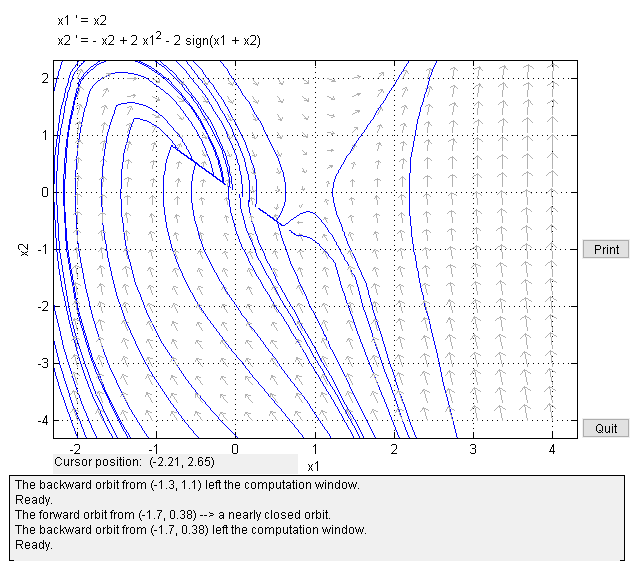
\includegraphics[width=0.8\textwidth]{lista2_8a.png}
    \caption{Diagrama de estados do sistema.}
    \label{fig:lista2_8a-png}
\end{figure}

\subexercise{b}

Evidentemente, a função candidata é positiva definida no ponto de equilíbrio proposto. Agora, vemos que 
\begin{align*}
    \dot{V} &= \nabla V f(x_1,x_2) = \begin{bmatrix} 
	x_1+x_2 & x_1+x_2
    \end{bmatrix} \begin{bmatrix} 
    x_2 \\
    -x_2 + 2x_1^2 -2 sign\left( x_1+x_2 \right) +u
    \end{bmatrix} \\
	    &= x_1x_2 + x_2^2 -x_1x_2 -x_2^2 +2x_1^2\left( x_1+x_2 \right)  -2\left( x_1+x_2 \right)  sign\left( x_1+x_2 \right) +u\left( x_1+x_2 \right) \\
	    &= \left( 2x_1^2 + u \right)\left( x_1+x_2 \right)   -2\left( x_1+x_2 \right)  sign\left( x_1+x_2 \right)
.\end{align*}
Assim, definindo $u = -2x_1^2 +sign\left( x_1+x_2 \right) $, temos \[
\dot{V} = -\left( x_1+x_2 \right)  sign\left( x_1+x_2 \right) = -\|h\|
,\] que é globalmente negativa definida para o equilíbrio em $(0,0)$,  ou seja, torna o equilíbrio GAE.

\begin{figure}[H]
    \centering
    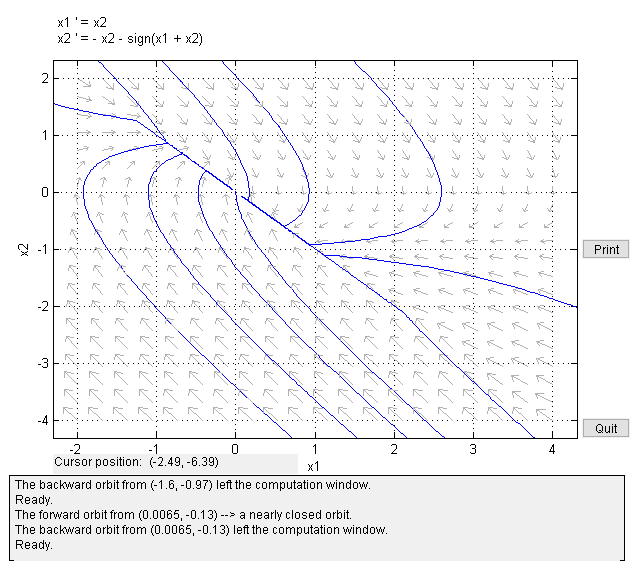
\includegraphics[width=0.8\textwidth]{lista2_8b.png}
    \caption{Diagrama de estados do sistema após projeto do controlador.}
    \label{fig:lista2_8b-png}
\end{figure}

\exercise{9}

\subexercise{a}

Podemos reescrever o lagrangiano do sistema como \[
\mathcal{L} = \frac{1}{2}m \dot{z}^2 - mgz
,\] que, pela equação de Euler-Lagrange, resulta em
\begin{align*}
    &\frac{\partial }{\partial t} \left( \frac{\partial \mathcal{L}}{\partial \dot{z}}  \right) = m \ddot{z} \\
    &\frac{\partial \mathcal{L}}{\partial z} = -mg \\
    &\implies m \ddot{z} +mg = F \\
    &\implies \ddot{z} = \frac{\alpha}{m}\left( u - \dot{z} \right)^2 - g
.\end{align*}

\subexercise{b}

Utilizando $x_1 = z$ e $x_2=\dot{z}$ podemo reescrever o sistema como \[
\begin{cases}
    \dot{x_1} = x_2 \\
    \dot{x_2} = \frac{\alpha}{m}\left( u-x_2 \right) ^2 - g
\end{cases}
.\]

\begin{figure}[H]
    \centering
    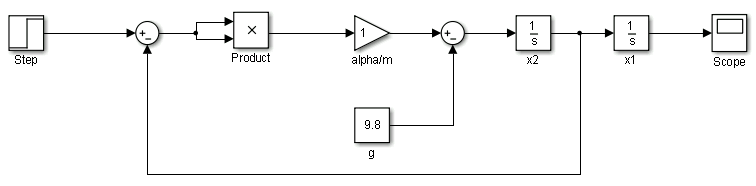
\includegraphics[width=0.8\textwidth]{lista2_9b.png}
    \caption{Diagrama de blocos do sistema. Bloco Step representa a entrada do controlador.}
    \label{fig:lista2_9b-png}
\end{figure}

Vemos que a dinâmica do sistema não depende da variável $x_1$, ou seja, independente da posição vertical em que ela se encontra, somente da sua variação.
\subexercise{c}

O equilíbrio do sistema pode ser encontrado por
\begin{align*}
    &\dot{x_1} = 0 \implies \overline{x_2} = 0 \\
    &\implies \frac{\alpha}{m}\overline{u}^2 = g \implies \overline{u} = \sqrt{\frac{\alpha g}{m}} 
,\end{align*}
para todo valor de $\overline{x_1}$

Analisamos a estabilidade do equilíbrio pela jacobiana, \[
    J(\overline{x_1},0) = \begin{bmatrix} 
    0 & 1 \\
    0 & -2 \frac{\alpha}{m}\overline{u}
\end{bmatrix} 
,\] que possui autovalores $\lambda = 0$ e $\lambda = -2 \frac{\alpha}{m}\overline{u}$.

Como podemos ver pela figura abaixo, no ponto de equilíbrio a bola possui velocidade nula, como esperado, e a sua posição se mantém constante. Mantendo a velocidade do ar dentro do tubo constante, a velocidade da bola sempre diminuirá em módulo atingindo uma posição vertical de equilíbrio.

\begin{figure}[H]
    \centering
    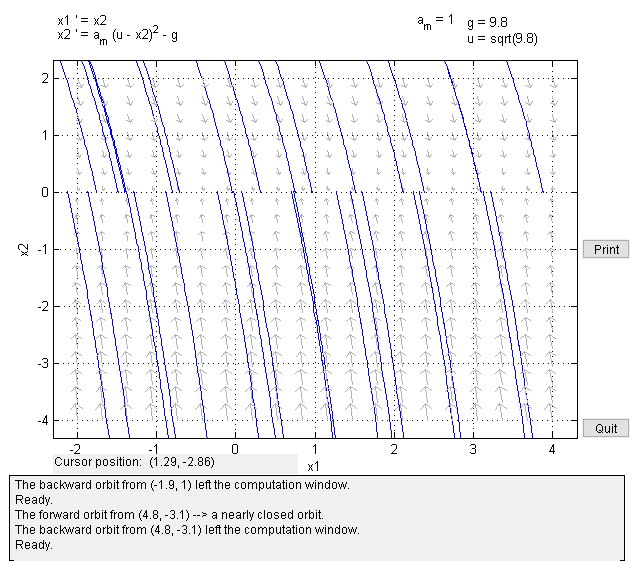
\includegraphics[width=0.8\textwidth]{lista2_9c.png}
    \caption{Diagrama de estados do sistema com $u(t) = \overline{u}$.}
    \label{fig:lista2_9c-png}
\end{figure}

\exercise{10}

\subexercise{a}

Considerando $y=x_1=z$, temos \[
\ddot{y} = \frac{\alpha}{m}\left( u -x_2 \right)^2 -g
,\] que nos permite implementar o método da realimentação linearizante como
\begin{align*}
    v &= \frac{\alpha}{m}\left( u -x_2 \right)^2 -g \\
      &\implies u = \sqrt{\frac{m\left( v +g \right) }{\alpha}} + x_2
,\end{align*}
tornando o sistema, do ponto de vista da nova entrada de controle, como \[
\ddot{y} = v
.\] 

\subexercise{b}

Para o sistema linearizado, podemos projetar uma lei de controle \[
v = \ddot{y_r} + k_0e + k_1\dot{e}
\] de forma que \[
\ddot{e} +k_0e + k_1\dot{e} = 0
,\] ou seja, queremos alocar os polos do polinômio característico \[
\lambda^2 + k_1\lambda + k_0 = 0
.\] 
Definindo $k_0=0$ e $k_1=2$ alocamos os polos coincidentes no valor fornecido no enunciado.

\subexercise{c}

Após garantido que o equilíbrio desejado é estável, devemos garantir que o sistema é estável internamente, ou seja, se durante o processo de linearização, os estados que não são mais observáveis continuam estáveis. O grau relativo do sistema é 2, portanto temos um comportamento de mesma ordem do sistema original.

\subexercise{d}

Se o parâmetro $m$ varia, o cancelamento deixa de ser preciso e o comportamento não linear do sistema se propaga para a saída. Uma possibilidade é projetar um estimador para o parâmetro $m$ e utilizá-lo no controle linearizante.

\exercise{11}

\subexercise{a}

Para o sistema \[
\begin{cases}
    \dot{x_1} = x_2 \\
    \dot{x_2} = v \\
    y = x_1
\end{cases}
,\] equivalente ao sistema após a realimentação linearizante, podemos projetar um controlador por estrutura variável \[
v = \begin{cases}
    1, &h(x_1,x_2) > 0 \\
    -1, &h(x_1,x_2) < 0
\end{cases}
,\] com $h\left( x_1,x_2 \right) =k_1\left( x_{1r}-x_1 \right) + k_2\left( 0-x_2 \right) $.

Vejamos que, com essa configuração, temos como condição para estabilidade que
\begin{align*}
    &\left< \nabla h, f^{+}\right> = -k_1x_2 -k_2 < 0\\
    &\left< \nabla h, f^{-}\right> = -k_1x_2 +k_2 > 0
,\end{align*}
ou seja, garantimos a estabilidade dentro de $x_2\in \left( -\frac{k_2}{k_1}, \frac{k_2}{k_1} \right) $.

Para o caso $h=0$, temos o sistema equivalente sobre a superfície de comutação, onde queremos fixar o ponto de equilíbrio com o controlador. Assim, analisamos \[
    \dot{h} = -k_1x_2 -k_2v_{eq} = 0 \implies v_{eq} = -\frac{k_1}{k_2}x_2
,\] portanto, o comportamento do sistema sobre a superfície de comutação é dado por \[
f_s = \begin{cases}
    x_2 \\
    -\frac{k_1}{k_2}x_2
\end{cases}
\] que claramente possui um equilíbrio em $(\overline{x_1},0)$. Como esse equilíbrio existe para $h(x_1,x_2)=0$, então podemos afirmar que ele é $(x_{1r},0)$. Ainda mais, como está dentro da região de deslizamento estável do sistema, esse é um equilíbrio estável.

\subexercise{b}

Conforme já exposto no item anterior.

\begin{figure}[H]
    \centering
    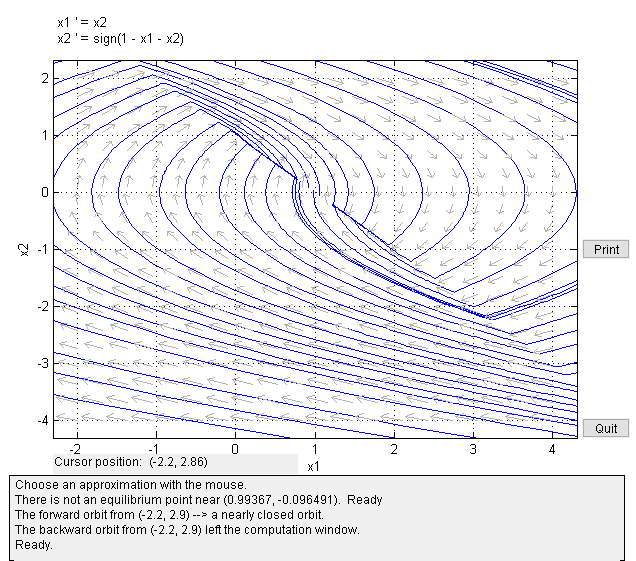
\includegraphics[width=0.8\textwidth]{lista2_11b}
    \caption{Diagrama de espaço de estados do sistema.}
    \label{fig:lista2_11b}
\end{figure}

\subexercise{c}

Uma ação de controle de um chaveamento de alta frequência será resultante. Para limitar a frequência de comutação, pode-se implementar um relé com histerese. Se deseja-se eliminar o chattering, pode-se aproximar o controlador como \[
v = \frac{h\left( x_1,x_2 \right) }{\sqrt{h\left( x_1,x_2 \right)^2 + 0.1^2} }
,\] por exemplo, dando uma resposta suave.

\exercise{12}

Vemos que
\begin{align*}
    \dot{V} &= \begin{bmatrix} -k_1\left( x_{1r}-x_1 \right)  & -k_2x_2\end{bmatrix} \begin{bmatrix} x_2 \\ \frac{\alpha}{m}\left( u-x_2 \right) ^2 -g \end{bmatrix} \\
    &= -k_1\left( x_{1r}-x_1 \right) x_2 -k_2 \frac{\alpha}{m}\left( u-x_2 \right)^2x_2 +gk_2x_2 \\
    &= \left( gk_2 -k_1\left( x_{1r}-x_1 \right) -k_2 \frac{\alpha}{m}\left( u-x_2 \right)^2 \right) x_2
.\end{align*}
Garantindo que \[
gk_2 -k_1\left( x_{1r}-x_1 \right) -k_2 \frac{\alpha}{m}\left( u-x_2 \right)^2 = -x_2\left(1 + \left( x_{1r} - x_1 \right)^2   \right) 
,\] temos \[
\dot{V} = -x_2^2 -x_2^2\left( x_{1r}-x_1 \right)^2
,\] o que indica a estabilidade assintótica do sistema no ponto de equilíbrio.

Assim, podemos primeiro transformar \[
u = v + x_2
,\] para simplificar a equação original para \[
gk_2 -k_1\left( x_{1r}-x_1 \right) -k_2 \frac{\alpha}{m}v^2 = -x_2\left(1 + \left( x_{1r} - x_1 \right)^2   \right)
.\] Portanto, basta definir o controlador como \[
v = \sqrt{ \frac{-m}{k_2\alpha}\left[  -x_2\left(1 + \left( x_{1r} - x_1 \right)^2   \right) - gk_2 +k_1\left( x_{1r}-x_1 \right)\right] }
.\] 

\exercise{13}

A energia do sistema pode ser utilizada como \[
    E = \frac{1}{2}m x_2^2 + mgx_1
\] temos uma função que não é positiva definida, portanto não pode ser utilizada como função de Lyapunov. Naturalmente, a energia no ponto de equilíbrio é $E_r = mgx_{1r}$.

Podemos, então, utilizar como função candidata de Lyapunov \[
V = \frac{1}{2}\left( E-E_r \right)^2 
,\] que é positiva definida para o ponto de equilíbrio. Assim,
\begin{align*}
    \dot{V} &= \left( E-E_r \right) \dot{E} \\
    \dot{E} &= mx_2\dot{x_2} +mg \dot{x_1} = mx_2\left( \frac{\alpha}{m}\left( u-x_2 \right)^2 -g \right) + mgx_2 \\
    &= \alpha x_2 \left( u-x_2 \right)^2 \\
    \implies \dot{V} &= (E-E_r)\alpha x_2 \left( u-x_2 \right)^2
.\end{align*}
Entretanto, veja que a ação do controle nunca poderá inverter o sinal do resto da equação, uma vez que está elevada ao quadrado, portanto, esse controle é impossível de ser efetuado.

\exercise{14}

\subexercise{a}

Escolhendo como estados \[
\bm{x} = \begin{bmatrix} y \\ \dot{y} \\ i \end{bmatrix} 
,\] podemos formular o sistema como \[
\begin{cases}
    \dot{x_1}= x_2 \\
    \dot{x_2} = g - \frac{k}{m}\left( \frac{x_3}{x_1} \right) ^2 \\
    \dot{x_3} = \frac{1}{L}v - \frac{R}{L}x_3
\end{cases}
.\] 

\begin{figure}[H]
    \centering
    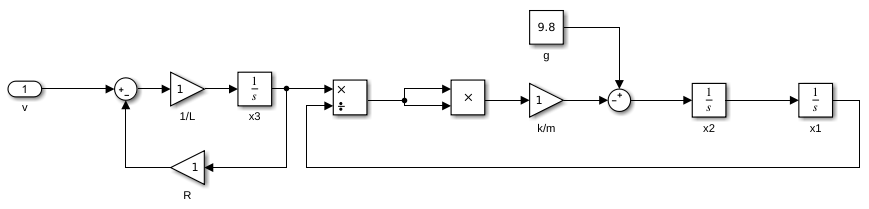
\includegraphics[width=0.8\textwidth]{lista2_14a.png}
    \caption{Diagrama de blocos do sistema.}
    \label{fig:lista2_11a-png}
\end{figure}

\subexercise{b}

Assumindo tal, temos pela equação (2) que \[
i = \frac{1}{R}v
,\] portanto podemos reescrever a equação (1) e, refazendo o sistema por variáveis de estado conforme o item anterior, chega-se em \[
\begin{cases}
    \dot{x_1} = x_2 \\
    \dot{x_2} = g - \frac{k}{mR^2}\left( \frac{v}{x_1} \right)^2
\end{cases}
.\] 

\subexercise{c}

No equilíbrio,
\begin{align*}
    \dot{x_1} = 0 &\implies \overline{x_2} = 0 \\
    \dot{x_2} = 0 &\implies \left( \frac{v}{\overline{x_1}} \right)^2 = \frac{mgR^2}{k} \\
		  &\implies \frac{v}{\overline{x_1}} = R \sqrt{\frac{mg}{k}} 
,\end{align*}
ou seja, assumindo que os coeficientes são todos unitários, $\overline{x_1} = \pm \overline{v}$. Pela jacobiana do sistema nesses equilíbrios, \[
    J(\pm v, 0) = \begin{bmatrix}
    0 & 1 \\
    1-\frac{v}{\overline{x_1}^2} & 0
\end{bmatrix} = \begin{bmatrix} 
    0 & 1 \\
    1 \pm \frac{1}{v} & 1
\end{bmatrix}
,\] que nunca possuirá autovalores negativos, ou seja, não são estáveis. Isso pode ser observado na figura abaixo.

\begin{figure}[H]
    \centering
    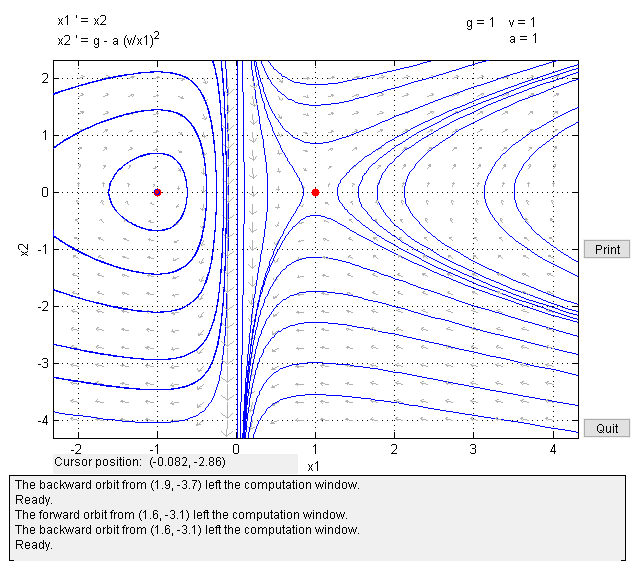
\includegraphics[width=0.8\textwidth]{lista2_14c.png}
    \caption{Diagrama de espaço de estados do sistema. Constantes unitárias e $v=1$.}
    \label{fig:lista2_14c-png}
\end{figure}

\exercise{15}

\subexercise{a}

Para o sistema reduzido, temos \[
y = x_1 \implies \dot{y} = x_2 \implies \ddot{y} = \dot{x_2} = g - \frac{k}{mR^2}\left( \frac{v}{x_1} \right)^2
,\] portanto, podemos projetar um novo sinal de controle virtual $u$ tal que \[
u = \ddot{y} \implies v(t) = x_1(t) R \sqrt{\frac{m}{k}\left( g-u(t) \right) } 
.\]

\subexercise{b}

Para garantir que o erro do sistema é zerado e se comporta de forma assintoticamente estável, formulamos o nosso novo sinal de controle $u$ \[
u(t) = \ddot{y_r}(t) + k_0e(t) + k_1\dot{e}(t)
,\] o que implica \[
\ddot{e}(t) = \ddot{y_r}(t) - \ddot{y}(t) \implies \ddot{e}(t) + k_1\dot{e}(t) + k_2e(t) = 0
.\] Podemos então controlar a dinâmica do erro $e(t)$ através das raízes do polinômio característico \[
\lambda^2 + k_1 \lambda + k_0 = 0
.\] Assim, calcula-se que ganhos $k_1=0.2$ e $k_0=0.01$ resultam em um sistema com os polos de malha fechada desejados.

\subexercise{c}

A estabilidade do sistema após ação da realimentação linearizante deve ser estudada para além da estabilidade do ponto de equilíbrio. Deve ser estudada a estabilidade da dinâmica interna, que é a parte do sistema que se torna não observável quando o grau relativo do sistema linearizado se torna menor do que o grau original do sistema. Não é o caso para este sistema, uma vez que após linearização ainda possui grau 2.

\subexercise{d}

vide questão 10, item d.

\exercise{16}

Para fins práticos, reescreve-se o sistema após linearização com estados $y_1 = y$ e $y_2=\dot{y}$.

Supondo um controlador de forma \[
    u(t) = sign(h) \text{ t.q. } h(y_1,y_2) = k_1\left( y_{r}-y_1 \right) +k_2(0-y_2)
,\] podemos projetar um controlador tal que o ponto de equilíbrio seja um pseudo-equilíbrio do sistema sobre a superfície $h\left( y_1,y_2 \right) =0$.

Sabemos que \[
\dot{h} = -k_1\dot{y_1} - k_2\dot{y_2} = -k_1y_2 - k_2u_{eq} = 0 \implies u_{eq} = -\frac{k_1}{k_2}y_2
,\] o que implica no sistema equivalente \[
f_s = \begin{bmatrix} 
    \dot{y_1} \\ \dot{y_2}
\end{bmatrix} = \begin{bmatrix} 
y_2 \\
u_{eq}
\end{bmatrix} = \begin{bmatrix} 
y_2 \\
-\frac{k_1}{k_2}y_2
\end{bmatrix} 
.\] É evidente que o ponto de pseudo-equilíbrio é da forma $(y_1,0)$, entretanto, como sabemos que ele se dá sobre a superfície $h(y_1,y_2) = 0$, podemos afirmar que ele é $\left( y_r, 0 \right)$.

Analisamos a estabilidade do equilíbrio pelo comportamento dos campos vetoriais, ou seja, garantindo que
\begin{align*}
    \left< \nabla h, f^{+} \right> = -k_1y_2 - k_2 < 0 \\
    \left< \nabla h, f^{-} \right> = -k_1y_2 + k_2 > 0 \\
.\end{align*}
É fácil ver que essas condições são verdadeiras para $y_2 \in  \left( -\frac{k_2}{k_1}, \frac{k_2}{k_1} \right) $, portanto, o ajuste dessas constantes impactará somente no tamanho da zona de deslizamento.

\subexercise{b}

Tanto o comportamento, o diagrama e o funcionamento são idênticos ao da questão 11.

\exercise{17}

Primeiro, vemos que \[
    E_0 = mg(y_{max} - y_r)
,\] e, portanto, \[
E - E_0 = \frac{1}{2}m \dot{y}^2 + mg\left( y_r - y \right) 
.\] Assim, \[
\dot{V} = \left( \frac{1}{2}m \dot{y}^2 + mg\left( y_r -y \right) \right) \left( m\dot{y}\ddot{y} - mg\left( y_r-y \right)\dot{y}  \right) = m^2 \left( \frac{1}{2} \dot{y}^2 + g\left( y_r -y \right) \right) \left( u - g\left( y_r-y \right)\right)\dot{y}
\] \[
\implies \dot{V} = \left( E-E_0 \right) \left( u-g\left( y_r-y \right)  \right) m\dot{y}
,\] ou seja, precisamos escolher $u$ de forma que a função $\dot{V}$ seja negativa definida. Veja que, se \[
\left( u-g\left( y_r - y \right)  \right) \dot{y} = -\left( E-E_0 \right) \|\dot{y}\|
,\] garantimos que $\dot{V}$ seja negativa definida. Assim, determinamos
\begin{align*}
    u &= -\left( E-E_0 \right) sign\left( \dot{y} \right) + g\left( y_r - y \right) \\
    \implies \dot{V} &= \left( E-E_0 \right) \left( -\left( E-E_0 \right) sign\left( \dot{y} \right) + g\left( y_r - y \right)-g\left( y_r-y \right)  \right) m\dot{y} \\
		     &= m\left( E-E_0 \right) \left( -\left( E-E_0 \right) sign(\dot{y}) \right) \dot{y} \\
		     &= -m\left( E-E_0 \right)^2 sign(\dot{y})\dot{y} \\
		     &= -m\left( E-E_0 \right)^2\|\dot{y}\| < 0 \forall (y,\dot{y}) \neq (y_r,0)
,\end{align*}
como se desejava.

\exercise{19}

A superfície de comutação é dada por \[
h\left( x_1,x_2 \right)  = x_1-x_{1r} + x_2-x_{2r} = 0
,\] variando o valor do controle $u$.

Podemos determinar a região de deslizamento atrativa a partir de
\begin{align*}
    &\left< \nabla h, f^{+}\right> = -x_2 + x_1 - \frac{1}{R}x_2 < 0 \\
    &\implies x_2 > \frac{R }{R+1}x_1 \\
    &\left< \nabla h, f^{-}\right> = -x_2 + E + x_1 - \frac{1}{R}x_2 > 0 \\
    &\implies x_2 < \frac{R }{R+1}\left( x_1+E \right)
,\end{align*}
ou seja, sabendo que a superfície de comutação nos restringe a \[
x_1 = x_{1r} + x_{2r} - x_2
\] e que $x_{2r} = 0.5 E$, temos
\begin{align*}
    &x_2 < \frac{R }{R+1}\left( x_1+E \right) \\
    &\implies x_2 < \frac{R}{2R + 1}\left( x_{1r} + 1,5 E \right) \\
    &x_2 > \frac{R }{R+1}x_1 \\
    &\implies x_2 > \frac{R}{2R + 1}\left( x_{1r} + 0,5 E \right)
.\end{align*}
Essas inequações definem a região de deslizamento da superfície de comutação.

\subexercise{b}

Temos, para a região com sinal positivo da função da superfície, \[
f^{+} = \begin{bmatrix} 
    -x_2 \\
    x_1 - \frac{1}{R}x_2
\end{bmatrix} 
,\] que possui equilíbrio $(0,0)$, ou seja, virtual, dado que $h(0,0)<0$.

Para a região com sinal negativo da função da superfície, \[
f^{-} = \begin{bmatrix} 
    -x_2 + E \\
    x_1 - \frac{1}{R}x_2
\end{bmatrix} 
,\] que possuirá equilíbrio em $(\frac{E}{R},E)$, ou seja, um equilíbrio real e estável somente se \[
x_{1r} > E\left( \frac{1}{R}+\frac{1}{2} \right) 
.\]

Para a superfície de comutação, podemos encontrar
\begin{align*}
    \dot{h} &= \dot{x_1} + \dot{x_2}  = 0 \\
	    &= -x_2 + Eu_{eq} + x_1 - \frac{1}{R}x_2 \\
    &\implies E u_{eq} = x_2 +\frac{1}{R}x_2 - x_1  \\
    &\implies f_s = \begin{bmatrix} 
	\frac{1}{R}x_2 - x_1  \\
	x_1 - \frac{1}{R}x_2
    \end{bmatrix}  \\
    &\implies \overline{x_1} = \frac{1}{R}\overline{x_2}
.\end{align*}
Sabendo que o equilíbrio está sobre a superfície de comutação, ou seja, \[
\overline{x_1}-x_{1r} + \overline{x_2} - x_{2r} = 0
,\] podemos determinar o equilíbrio do sistema na superfície de comutação em
\begin{align*}
    &x_{1r} - \overline{x_2} + x_{2r} = \frac{1}{R}\overline{x_2} \\
    &\implies \overline{x_2} = \frac{R}{R+1}\left( x_{1r} + 0,5 E \right) \\
    &\implies \overline{x_1} = \frac{1}{R+1}\left( x_{1r} + 0,5 E \right) 
,\end{align*}
valores que respeitam as condições de estabilidade previamente calculadas.

\subexercise{c}

\begin{figure}[H]
    \centering
    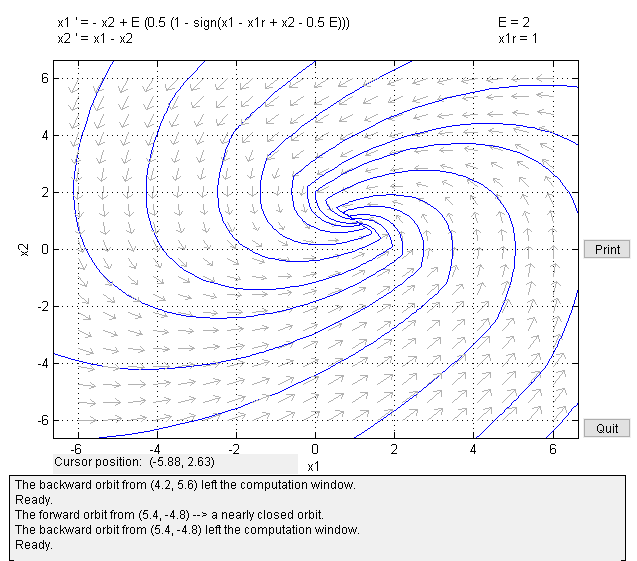
\includegraphics[width=0.8\textwidth]{lista2_19c.png}
    \caption{Diagrama de estados do sistema com $R=1$.}
    \label{fig:lista2_19c-png}
\end{figure}

\exercise{20}

\subexercise{a}

Dado o sistema, temos
\begin{align*}
    &\dot{y} = \dot{x} = -x_1^3 -x_2 \\
    &\ddot{y} = -3x_1^2 \dot{x_1} -\dot{x_2} = -3x_1^2\left( -x_1^3-x_2 \right) +x_1 +x_2^3 + u \\
    &\implies \ddot{y} = 3x_1^{5} + 3x_1^2x_2 + x_1 + x_2^3 + u
.\end{align*}
Assim, para linearizar a saída desse sistema, definimos uma nova entrada $v$ de forma que
\begin{align*}
    &v = 3x_1^{5} + 3x_1^2x_2 + x_1 + x_2^3 + u \\
    &\implies u = v - 3x_1^{5} - 3x_1^2x_2 - x_1 - x_2^3
.\end{align*}

\subexercise{b}

O sistema linearizado pode ser visto como \[
\ddot{y} = v
,\] o que nos permite definir, pensando em atingir erro nulo, \[
\dot{v} = \dddot{y_r} + k_0e + k_1\dot{e} + k_2 \ddot{e}
.\] O que implica na dinâmica do erro tal que \[
e = y_r - y \implies \dddot{e} = \dddot{y_r} - \dot{v} \implies \dddot{e} + k_2 \ddot{e}+ k_1\dot{e} + k_0e = 0
.\] Através do polinômio característico da dinâmica do erro podemos ajustar os ganhos para que os polos sejam alocados nas posições desejadas. Temos \[
\lambda^3 + k_2\lambda^2 + k_1\lambda + k_0 = 0
.\] Se quisermos que as raízes sejam -1 e -2, então 
\begin{align*}
    \lambda^3 + k_2\lambda^2 + k_1\lambda + k_0 &= \left( \lambda + 1 \right)^2\left( \lambda +2 \right) \\
						&= \lambda^3 + 4\lambda^2 + 5\lambda + 1
,\end{align*}
ou seja, $k_2=4$, $k_1=5$ e $k_0=1$.

\subexercise{c}

Para definir os parâmetros da lei de controle, assumimos que o sistema é estável no equilíbrio proposto e calculamos os parâmetros que fazem com que a função candidata de Lyapunov seja tal que $\dot{V}$ seja negativa definida, além de, claro, $V$ ser positiva definida, no equilíbrio.

Então, temos que 
\begin{align*}
    \dot{V} &= h \dot{h} = h \left( -k_1\dot{x_1} -k_2\dot{x_2} \right) \\
	    &= h \left( -k_1\left( -x_1^3 -x_2 \right) -k_2\left( -x_1-x_2^3+u \right) \right)
.\end{align*}
Veja que se \[
    -k_1\left( -x_1^3 -x_2 \right) -k_2\left( -x_1-x_2^3+u \right) = -h
,\] então $\dot{V} = -h^2$. Para isso, basta que \[
u = \frac{h - k_1\left( -x_1^3 -x_2 \right)}{k_2} + x_1 + x_2^3
.\] Assim temos um equilíbrio global assintoticamente estável.

\exercise{21}

\subexercise{a}

Dada a função candidata enunciada, temos 
\begin{align*}
    \dot{V} &= \frac{1}{2}\left( 2z\dot{z} + 2\dot{z}\ddot{z} \right) \\
	    &= \frac{1}{2}\dot{z} \left( 2z + 2\left( u -z -\dot{z}\left( z^2 -1 \right)  \right)  \right) \\
	    &= \frac{1}{2}\dot{z} \left(  2u -2\dot{z}\left( z^2 -1 \right)  \right) \\
	    &= \frac{1}{2}\dot{z} \left(  2u +2\dot{z}\right) - \dot{z}^2z^2 \\
.\end{align*}
veja que, se $u = -\dot{z}$, então \[
\dot{V} = -\dot{z}^2z^2
,\] portanto, o equilíbrio é globalmente assintoticamente estável.

\subexercise{b}

Reescrevendo o sistema na forma \[
\ddot{z} = u -z -\dot{z}\left( z^2 -1 \right)
\] fica claro ver que, se tivermos um controle tal que \[
v = u -z -\dot{z}\left( z^2 -1 \right) \implies u = v +z +\dot{z}\left( z^2 -1 \right)
,\] então o sistema poderá ser controlado como um duplo integrador.

Para o controle do sistema, um controlador PD simples com ganho $k_p = 60$ e $k_d = 15$, por exemplo, estaria dentro das especificações. Considerando uma implementação paralela.

\exercise{22}

Sabemos que o volume de líquido no tanque pode ser descrito por
\begin{align*}
    V &= A(h) \frac{h}{3} \\
      &= \frac{\pi d(h)^2}{4}\frac{h}{3} \\
      &= \frac{\pi}{4}\frac{36}{100}\frac{h^3}{3} = \frac{3\pi}{100}h^3
.\end{align*}

Agora, sabendo que os fluxos podem ser determinados a partir de
\begin{align*}
    \dot{V} &= q_1-q_2 \\
	    &= q_1 - A_2\sqrt{2gh} 
\end{align*}
e
\begin{align*}
    \dot{V} &= \frac{9\pi}{100}h^2 \dot{h}
,\end{align*}
portanto, podemos definir \[
    \dot{h} = \frac{100\left( u - A_2\sqrt{2gh}  \right) }{9\pi h^2}
,\] um sistema de primeiro grau onde $h$ é o estado.


\subexercise{b}

Define-se um sinal de controle virtual $v$ com o objetivo que $\dot{y} = v$, linearizando o sistema. Para isso,
\begin{align*}
    &v = \frac{100\left( u - A_2\sqrt{2gh}  \right) }{9\pi h^2} \\
    &\implies \frac{9\pi x_1^2 v}{100} = u - A_2\sqrt{2gh} \\
    &\implies u = \frac{9\pi x_1^2 v}{100} + A_2\sqrt{2gh}
.\end{align*}

\subexercise{c}

Esse método depende da precisa estimativa dos parâmetros do modelo, por exemplo, se o parâmetro $A_2$ não estiver precisamente estimado, o sistema terá um comportamento não linear para o qual o controle não está projetado.

\subexercise{d}

O problema de saturação é conhecido por implicar em uma maior inércia ao controlador quando fora dos limites de saturação. Métodos de anti-windup podem ser aplicados, realimentando o valor acima da saturação para a ação de controle.

\subexercise{e}

Com um estimador de estados, que funciona como uma réplica virtual da planta que estima o valor do parâmetro desconhecido a partir da modelagem.

\exercise{23}

Os campos podem ser modelados pelas equações
\begin{align*}
    f^{+} &= \begin{bmatrix} 
	-x^3 -y \\
	-x -y^3 -1
    \end{bmatrix} \\
    f^{-} &= \begin{bmatrix} 
	-x^3 -y \\
	-x -y^3 +1
    \end{bmatrix}
.\end{align*}

Sabendo que \[
    \nabla h = \begin{bmatrix} -1 & 1 \end{bmatrix} 
,\] a superfície de deslizamento pode ser determinada como a região da superfície $h(x,y) = 0$ que satisfaz as inequações
\begin{align*}
    \left< \nabla h, f^{+} \right> = x^3 + y -x -y^3 -1 <0 \\
    \left< \nabla h, f^{-} \right> = x^3 + y -x -y^3 +1 >0
.\end{align*}

O comportamento na superfície $h(x,y)=0$ pode ser determinado a partir de
\begin{align*}
    &\dot{h} = \dot{y} - \dot{x} = -x -y^3 -u_{eq} + x^3 + y = 0 \\
    &\implies u_{eq} = -x -y^3 + x^3 + y \\
    &\implies f_s = \begin{bmatrix} 
	-x^3 -y \\
	-x -y^3 -u_{eq}
    \end{bmatrix} = \begin{bmatrix} 
	-x^3 -y \\
	-x^3 -y
\end{bmatrix} 
.\end{align*}

Os equilíbrios dos campos vetoriais podem ser determinados tendo que \[
    \dot{x} = 0 \implies \overline{y} = -\overline{x}^3
,\] então, para $f^{+}$,
\begin{align*}
    &\dot{y}  = \overline{x}^{9} - \overline{x} -1 = 0 \\
    &\implies \overline{x} \cong 1,08507 \implies \overline{y} \cong -1,27754
\end{align*}
e para $f^{-}$,
\begin{align*}
    &\dot{y}  = \overline{x}^{9} - \overline{x} +1 = 0 \\
    &\implies \overline{x} \cong -1,08507 \implies \overline{y} \cong 1,27754
.\end{align*}
Vemos que ambos são equilíbrios virtuais.

Em relação ao sistema sobre a superfície de comutação, vê-se que
\begin{align*}
    \overline{y} = -\overline{x}^3 \\
    h(\overline{x},\overline{y}) = 0 \implies \overline{x} = \overline{y} \\
    \implies \overline{y} = -\overline{y}^3 \implies \overline{y} = \overline{x} = 0
.\end{align*}
Vemos que \[
    J_{f_s}(0,0) = \begin{bmatrix} 
    -3\overline{x}^3 & -1 \\
    -3\overline{x}^3 & -1
\end{bmatrix} = \begin{bmatrix} 
    0 & -1 \\
    0 & -1 \\
\end{bmatrix}
,\] que possui autovalores $\left\{ 0, -1 \right\}$, ou seja, é um equilíbrio crítico.

\begin{figure}[H]
    \centering
    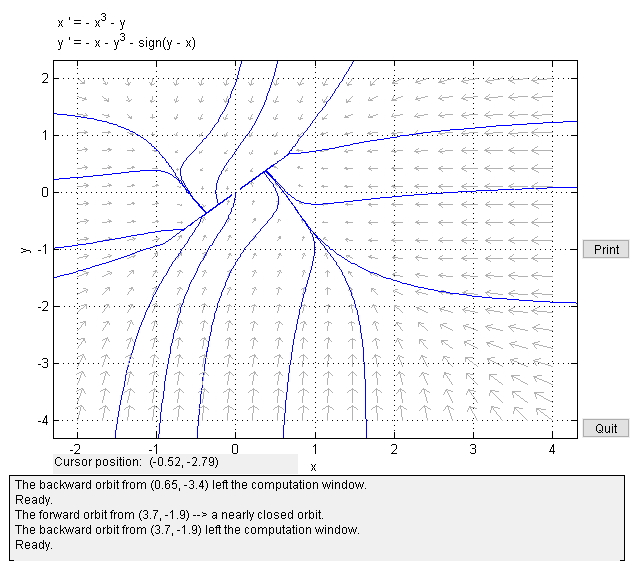
\includegraphics[width=0.8\textwidth]{lista2_23.png}
    \caption{Espaço de estados do sistema.}
    \label{fig:lista2_23-png}
\end{figure}

\exercise{24}

\subexercise{a}

Primeiro deriva-se a relação entre a saída e o sinal de controle
\begin{align*}
    \dot{x} &= -x^3 - y \\
    \implies \ddot{x} &= -3x \dot{x} -\dot{y} \\
		      &= -3x \left( -x^3 - y \right) +x +y^3 +u(t)
.\end{align*}
Então, para que tenhamos uma relação linear $v(t) = \ddot{x}(t)$, fazemos
\begin{align*}
    v &= -3x \left( -x^3 - y \right) +x +y^3 +u(t) \\
    \implies u &= v +3x \left( -x^3 - y \right) -x -y^3
.\end{align*}

\subexercise{b}

Pode-se projetar um controlador com uma ação integral \[
    \dot{v} = \dddot{x_r} + k_2\ddot{e}+ k_1\dot{e} + k_0 e
,\] fazendo com que
\begin{align*}
    &\dddot{e} = \dddot{x_r} - \dddot{x} \\
    &\implies \dddot{e}+ k_2\ddot{e}+ k_1\dot{e} + k_0 e = 0
.\end{align*}
Podemos estudar a estabilidade desse sistema através do polinômio característico \[
    \lambda^3 + k_2\lambda^2 + k_1\lambda + k_0 = 0
.\] Alocando os polos todos em -1, temos
\begin{align*}
    \lambda^3 + k_2\lambda^2 + k_1\lambda + k_0 &= \left( \lambda + 1 \right)^3 \\
						&= \lambda^3 + 3\lambda^2 + 3\lambda + 1
,\end{align*}
portanto $k_0=1$ e $k_1=k_2=3$.

\subexercise{c}

Após a linearização, o sistema possui grau relativo 2, mesmo que o sistema original, portanto não há estados não observáveis, ou seja, não há dinâmica interna. Assim, a estabilidade do sistema pode ser determinada pela dinâmica do sistema com o controlador, que como foi projetado para ter polos negativos, é estável.

\subexercise{d}

Determinamos a lei de controle pelos parâmetros $s_1$ e $s_2$ que fazem com que a função candidata de Lyapunov indique a estabilidade do sistema, ou seja, queremos que $\dot{V}$ seja negativa definida no ponto de equilíbrio.

Assim,
\begin{align*}
    \dot{V} &= h \dot{h} = h \left( -s_1\dot{x_1} -s_2\dot{x_2} \right) \\
	    &= h \left( -s_1\left( -x_1^3 -x_2 \right) -s_2\left( -x_1 -x_2^3 -u  \right)   \right) \\
	    &= h \left( s_1 x_1^{3} +s_2x_1 +s_2x_2^{3} +s_1x_2+s_2u  \right)  \\
.\end{align*}
Veja que se fizermos com que $\dot{V} = h sign(h) = \|h\|$, garantimos a estabilidade do sistema no ponto de equilíbrio. Para isso,
\begin{align*}
    s_1 x_1^{3} +s_2x_1 +s_2x_2^{3} +s_2x_2 +s_2u  = sign(h) \\
    \implies u = \frac{1}{s_2}sign(h) - \frac{s_1}{s_2} x_1^{3} -x_1 -x_2^{3} -\frac{s_1}{s_2}x_2
.\end{align*}

\exercise{25}

\subexercise{a}

Analisamos primeiro os equilíbrios dos campos vetoriais. Para $f^{+}$,
\begin{align*}
    \dot{x} = 0 &\implies x = 3y^2 \\
    \dot{y} = 0 &\implies 2x - y^3 -1 = 0 \\
		&\implies 6y^2 - y^3 - 1 = 0
,\end{align*}
com equilíbrios em $y \in  \left\{ -0,40, 0,42, 5,97 \right\}$, sendo somente $(0,48, -0,4)$ virtual, todos os outros dois reais.

Para $f^{-}$,
\begin{align*}
    \dot{y} = 0 &\implies 2x - y^3 +1 = 0 \\
		&\implies 6y^2 - y^3 + 1 = 0
,\end{align*}
ou seja, possui equilíbrio em $(108,99, 6,028)$, que é um equilíbrio virtual.

Para o sistema equivalente sobre a superfície de comutação  $h=0$, primeiro vemos
\begin{align*}
    \dot{h} =0&= \frac{1}{2}\dot{x} + \dot{y} \\
	      &= -\frac{1}{2}x + \frac{3}{2}y^2 +2x -y^3 + u_{eq} \\
    \implies u_{eq} &= -\frac{3}{2}x -\frac{3}{2}y^2 + y^3
,\end{align*}
assim, o sistema pode ser observado como \[
f_s = \begin{bmatrix} -x +3y^2 \\ \frac{1}{2}x -\frac{3}{2}y^2 \end{bmatrix} 
.\] 

\subexercise{b}

\begin{figure}[H]
    \centering
    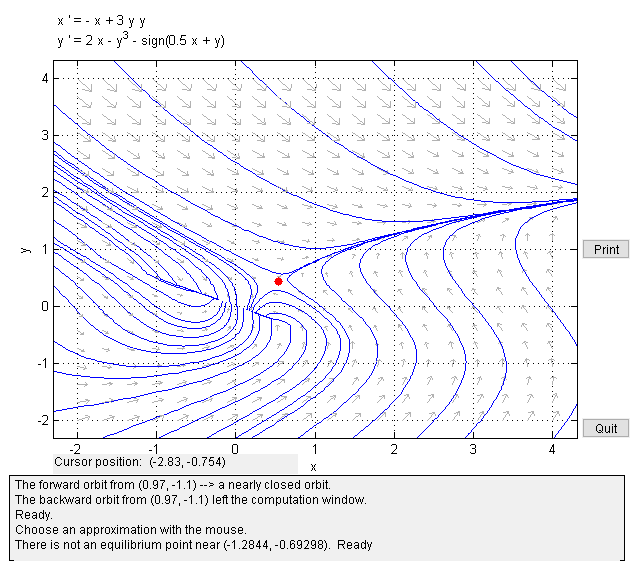
\includegraphics[width=0.8\textwidth]{lista2_25b_1.png}
    \caption{Diagrama de estados do sistema.}
    \label{fig:lista2_25b_1-png}
\end{figure}

\begin{figure}[H]
    \centering
    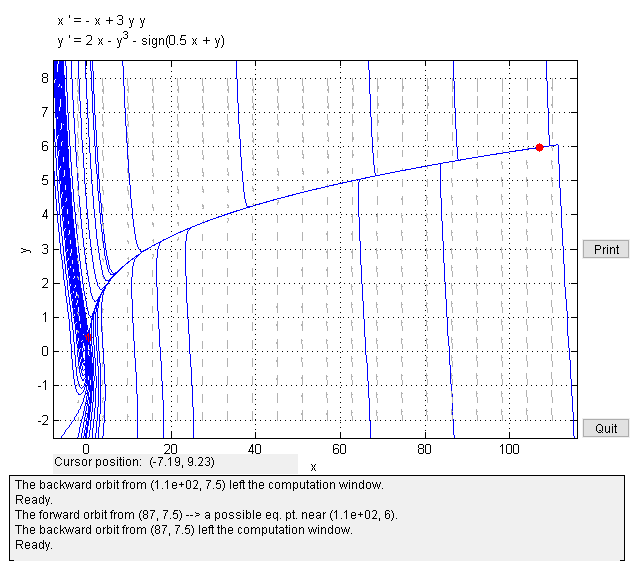
\includegraphics[width=0.8\textwidth]{lista2_25b_2.png}
    \caption{Diagrama de estados, mostrando o equilíbrio real e estávael do campo vetorial positivo.}
    \label{fig:lista2_25b_2-png}
\end{figure}

\exercise{26}

Para o sistema com superfície de comutação $h(x1,x_2) = 1+x_2 = 0$, podemos encontrar a região de deslizamento por 
\begin{align*}
    \left< \nabla h, f^{+} \right> = -x_1 -1 <0 \implies x_1 > -1 \\
    \left< \nabla h, f^{-} \right> = -x_1 +1 >0 \implies x_1 < 1
,\end{align*}
ou seja, a região de deslizamento é $x_1\in \left( -1,1 \right)$.

Equilíbrio de \[
f^{+} = \begin{bmatrix} x_2 \\ -x_1 -1 \end{bmatrix}
\] é em $(-1,0)$, ou seja, um equilíbrio real. Equilíbrio de \[
f^{-} = \begin{bmatrix} x_2 \\ -x_1 + 1 \end{bmatrix} 
\] em $(1,0)$, portanto, virtual.

Para o sistema equivalente sobre a superfície de comutação, primeiro vemos que \[
\dot{h} = -x_1 -u_{eq} = 0 \implies u_{eq} = -x_1
,\] o que resulta em \[
f_s = \begin{bmatrix} x_2 \\ -x_1 +x_1 \end{bmatrix} = \begin{bmatrix} x_2 \\ 0 \end{bmatrix} 
,\] ou seja, não possui equilíbrios na superfície de deslizamento.

\subexercise{b}

Com base no diagrama do espaço de estados apresentado, pode-se observar que como a superfície de comutação não possui equilíbrios, ela acaba somente fazendo com que o sistema apresente comportamento convergente para um ciclo limite ao redor do equilíbrio $(-1,0)$. Podemos controlar o "raio" desse ciclo limite através da constante da superfície de comutação, ou seja, se a superfície fosse $h(x_1,x_2) = 2 + x_2$, teríamos um ciclo limite com raio 2 em torno do ponto de equilíbrio.

\exercise{27}

Podemos linearizar o sistema com controle nulo como \[
    A(\bm{\overline{x}}) = \begin{bmatrix} 
	-3 +2a \overline{x_2}^2 & 4a\overline{x_1} \overline{x_2} \\
	-3a \overline{x_1}^2 & -2a +1
\end{bmatrix} = \begin{bmatrix} 
	-3 & 0 \\
	0 & -2a + 1
\end{bmatrix} 
.\] Podemos determinar a estabilidade desse equilíbrio através de seus autovalores, que são claramente $-3$ e $1-2a$. Ou seja, para que o sistema seja LAE,  \[
1-2a < 0 \implies a > \frac{1}{2}
.\] 

\subexercise{b}

Com o controle proposto, o sistema torna-se \[
f = \begin{bmatrix} -3x_1 + x_1^2x_2 \\ -x_1^3 -x_2 \end{bmatrix} 
.\] Assim, utilizando a função candidata de Lyapunov \[
V\left( \bm{x} \right) = \frac{1}{2}\|\bm{x}\|
,\] podemos computar
\begin{align*}
\dot{V} &= \nabla V \cdot f \\
&= \begin{bmatrix} x_1 & x_2 \end{bmatrix} \begin{bmatrix} -3x_1 + x_1^2x_2 \\ -x_1^3 -x_2 \end{bmatrix} \\
&= -3x_1^2 + x_1^3x_2 -x_1^3x_2 -x_2^3 \\
&= -3x_1^2 -x_2^3
.\end{align*}
Como vemos que $\dot{V}$ é negativa definida, o sistema é GAE no equilíbrio.

\exercise{28}

Para a função candidata de  Lyapunov, que claramente é positiva definida, vemos que 
\begin{align*}
    \dot{V} &= L \overline{x_1}\dot{x_1} + C \overline{x_2} \dot{x_2} \\
	    &= \overline{x_1}\left( E - ux_2 \right) + \overline{x_2} \left( ux_1 - \frac{1}{R}x_2 \right) \\
	    &= \overline{x_1}E -\overline{x_2}\frac{1}{R}x_2 + u\left( \overline{x_2}x_1 -\overline{x_1}x_2 \right) 
.\end{align*}
Considerando que $x_1,x_2 > 0$, podemos escolher \[
u = \begin{cases}
    \frac{u'}{\overline{x_2}x_1 -\overline{x_1}x_2} &\text{, }\bm{x} \neq \bm{\overline{x}} \\
    0 &\text{, }\bm{x} = \bm{\overline{x}}
\end{cases}
,\] o que implica em
\begin{align*}
    \dot{V} &= \overline{x_1}E -\overline{x_2}\frac{1}{R}x_2 + u'
.\end{align*}
Veja que essa abordagem já garante que $\dot{V}(\overline{x_1}, \overline{x_2}) = 0$. Agora, precisamos que \[
\overline{x_1}E -\overline{x_2}\frac{1}{R}x_2 + u' < 0
,\] portanto, escolhendo \[
u' = -\overline{x_1}E +\overline{x_2}\frac{1}{R}x_2 -u''
\] com $u'' = 1$ seria o suficiente. Para garantirmos suavidade no sistema, precisamos que
\begin{align*}
    0 &= \lim_{\bm{x} \to \overline{\bm{x}}} u \\
      &= \lim_{\bm{x} \to \overline{\bm{x}}} \frac{-\overline{x_1}E +\overline{x_2}\frac{1}{R}x_2 -u''}{\overline{x_2}x_1 -\overline{x_1}x_2} \\
      &= \lim_{\bm{x} \to \overline{\bm{x}}} \frac{-Ex_1 + x_{1e}E + \frac{1}{R}x_2^2 - x_{2e}\frac{1}{R}x_2 -u''}{x_{1e}x_2 - x_{2e}x_1}
.\end{align*}
Para isso, definimos \[
    u''(x_1,x_2) = u''_1(x_1) + u''_2(x_2)
\] e analisamos o limite em cada uma das dimensões, ou seja, 
\begin{align*}
     0 &= \lim_{x_1 \to \overline{x_1}} \frac{-Ex_1 + x_{1e}E + \frac{1}{R}x_2^2 - x_{2e}\frac{1}{R}x_2 -u''}{x_{1e}x_2 - x_{2e}x_1} \\
    &= \lim_{x_1 \to \overline{x_1}} \frac{-E - \frac{\partial u''}{\partial x_1} }{ -x_{2e} } \\
     \implies \frac{\partial u''}{\partial x_1} &= -E \implies u''_1 = -Ex_1
\end{align*}
e
\begin{align*}
     0 &= \lim_{x_2 \to \overline{x_2}} \frac{-Ex_1 + x_{1e}E + \frac{1}{R}x_2^2 - x_{2e}\frac{1}{R}x_2 -u''}{x_{1e}x_2 - x_{2e}x_1} \\
&= \lim_{x_2 \to \overline{x_2}} \frac{\frac{2}{R}x_2 -x_{2e}\frac{1}{R} - \frac{\partial u''}{\partial x_2} }{x_{1e}} \\
     \implies \frac{\partial u''}{\partial x_2} &= \frac{1}{R}\left( 2x_2 -x_{2e} \right) \implies u''_2 = \frac{1}{R}\left( x_2^2 -x_{2e}x_2 \right) = \frac{1}{R}\overline{x_2}x_2
.\end{align*}

Conclui-se que \[
u = \begin{cases}
    \frac{E \overline{x_1} +\overline{x_2}\frac{1}{R}x_2 -\frac{1}{R}x_2\overline{x_2} }{\overline{x_2}x_1 -\overline{x_1}x_2} &\text{, }\bm{x} \neq \bm{\overline{x}} \\
    0 &\text{, }\bm{x} = \bm{\overline{x}}
\end{cases}
\] garante a estabilidade assintótica do sistema no equilíbrio.

\exercise{29}

\subexercise{a}

Para linearizar a saída, desenvolvemos
\begin{align*}
    \dot{y} &= \dot{x_1} = x_1 - x_2x_3 \\
    \implies \ddot{y} &= \dot{x_1} -\dot{x_2}\dot{x_3} \\
		      &= x_1 -x_2x_3 -\left( x_3 -x_1x_3 \right) x_1u  \\
		      &= x_1 - x_2x_3 -x_1\left( 1-x_1 \right) x_3 u
.\end{align*}
Assim, se queremos linearizar o sistema de forma que $\ddot{y} = v$, então
\begin{align*}
    &v = x_1 - x_2x_3 -x_1\left( 1-x_1 \right) x_3 u \\
    & \implies x_1\left( 1-x_1 \right) x_3 u = x_1 - x_2x_3 - v \\
    & \implies u = \frac{x_1 - x_2x_3 - v}{x_1\left( 1-x_1 \right) x_3}
.\end{align*}

\subexercise{b}

O sistema linearizado possui grau relativo 2, ou seja, existe uma dinâmica interna de grau 1, uma vez que o sistema original é de grau 3.

\subexercise{c}

Para garantir o seguimento de referência, podemos projetar o controlador tal que \[
v = \ddot{y_r} + k_0e + k_1 \dot{e}
,\] o que nos permite calcular
\begin{align*}
    &e = y_r - y \\
    &\implies \ddot{e} = \ddot{y_r} - v \\
    &\implies \ddot{e} + k_1 \dot{e} + k_0 e = 0
.\end{align*}
Assim, analisando o polinômio característico \[
    \lambda^2 + k_1\lambda + k_0 = 0
\] podemos escolher $k_0 = 6$ e $k_1 = 5$ para alocar os autovalores em $-3$ e $2$.

\subexercise{d}

Dinâmica interna representa a dinâmica do sistema inicial que tornou-se não observável após o controle linearizante. Sua estabilidade é importante pois garante a estabilidade do sistema como um todo.

\exercise{30}

Primeiro, rearranjamos o sistema \[
\ddot{\theta} = \sin \theta \left( u \cos\theta - 1 \right) - \dot{\theta}
\] escolhendo os estados como $x_1 = \theta$ e $x_2 = \dot{\theta}$, de forma que \[
\begin{cases}
    \dot{x_1} = x_2 \\
    \dot{x_2} = \sin x_1 \left( u \cos x_1 -1 \right) -x_2
\end{cases}
.\] 

Agora, consideramos uma modificação da superfície de comutação em torno da referência, ou seja, $h\left( \bm{x} \right) = s_1(x_1-x_{1r}) +s_2x_2$. Podemos, agora, determinar o controle através da estabilidade do sistema utilizando a função candidata de Lyapunov \[
V = \frac{1}{2}h^2
.\] Assim, vemos que
\begin{align*}
    \dot{V} &= h \dot{h} = h \left( s_1\dot{x_1} + s_2 \dot{x_2} \right) \\
	    &= h(s_1x_2 -s_2\sin x_1 -s_2x_2 + s_2 \sin x_1 \cos x_1 u)
.\end{align*}
Escolhendo \[
u = \frac{1}{s_2 \sin x_1 \cos x_1}v 
,\] temos
\begin{align*}
    \dot{V} &= h(s_1x_2 -s_2\sin x_1 -s_2x_2 + v )
.\end{align*}
Desta forma, basta definir \[
    v = -s_1x_2 +s_2\sin x_1 +s_2x_2 - sign(h)
,\] que teremos \[
\dot{V} = -\|h\|
,\] ou seja, garantimos que o sistema é estável no ponto de equilíbrio.

Podemos determinar a região de estabilidade do sistema pela região de deslizamento do sistema, ou seja, pelas condições
\begin{align*}
    &\left< \nabla h, f^{+} \right> = s_1x_2 -s_2\sin x_1 -s_2x_2 + s_2 \sin x_1 \cos x_1 u = -1 <0 \\
    &\left< \nabla h, f^{-} \right> = 1 >0
,\end{align*}
i.e., o sistema é globalmente estável, dentro do intervalo para o qual o controlador está definido $x_1 \in \left( 0, \frac{\pi}{2} \right) $.

\end{document}
